\chapter{Tổng quan về n8n}

\section{n8n là gì?}

\begin{figure}[htbp]
    \centering
    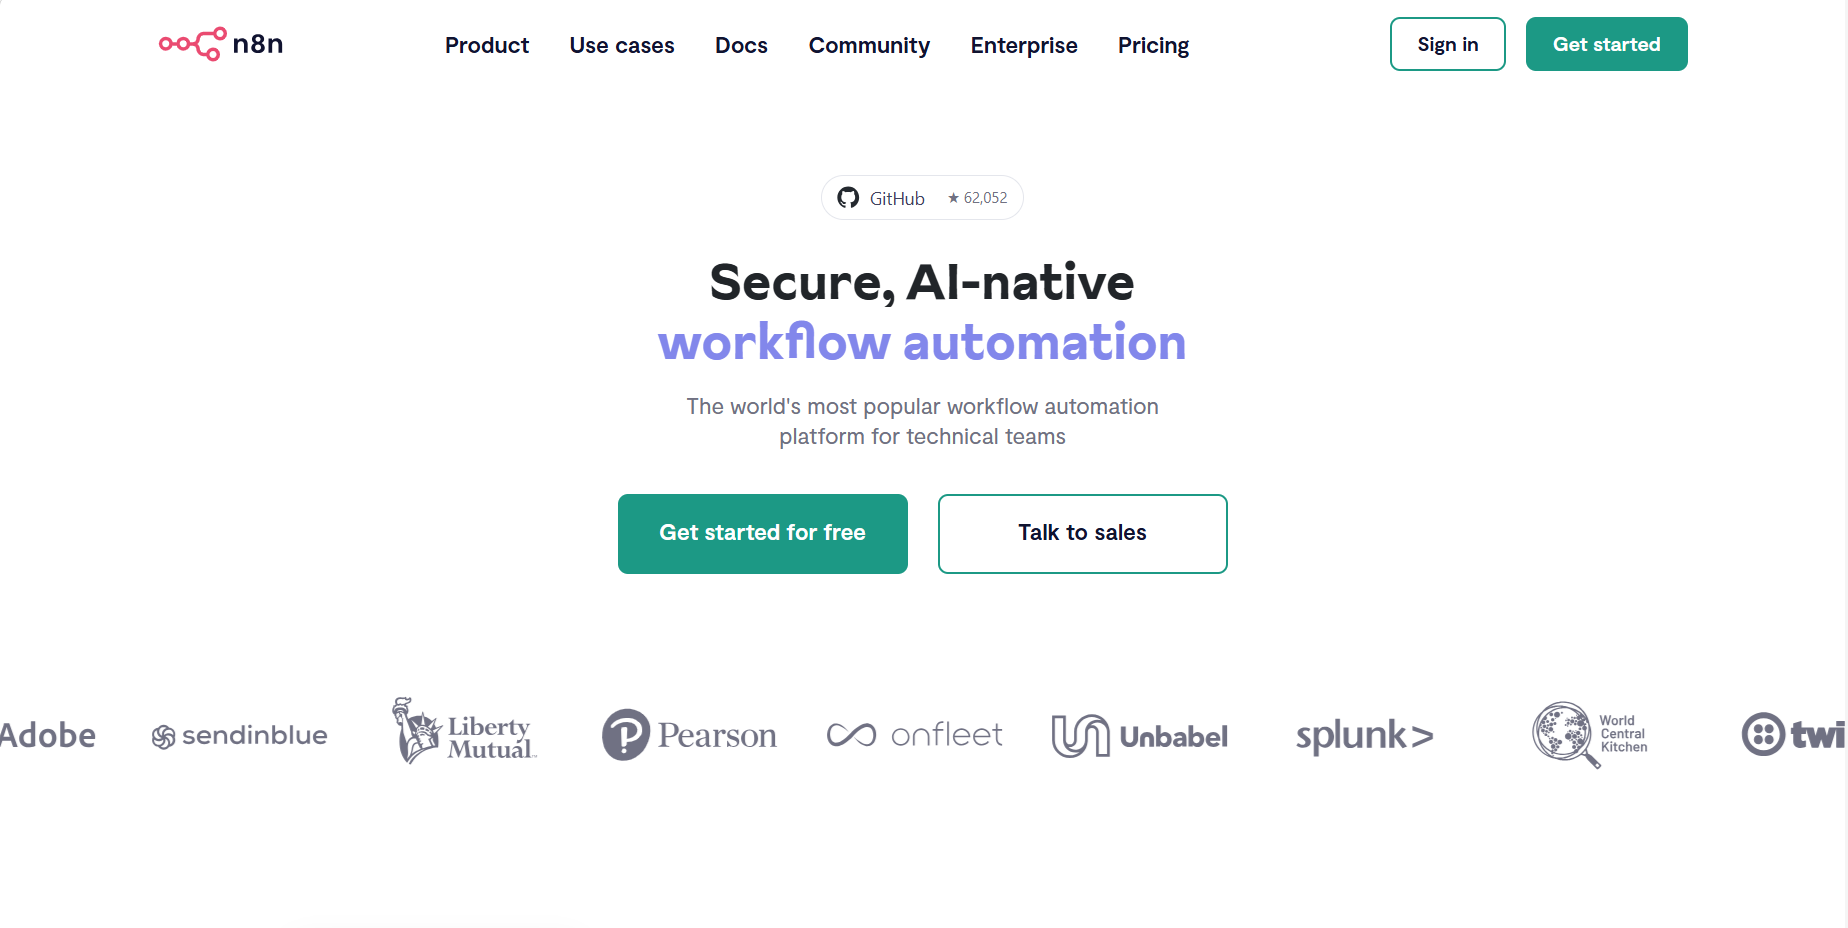
\includegraphics[width=1\linewidth]{images/n8n.png}
    \caption{Trang chủ n8n}
\end{figure}

Có bao giờ bạn mong ước mình chỉ cần "vẽ " vài đường đơn giản là có thể dựng nên cả một hệ thống tự động hóa phức tạp chỉ bằng vài cú nhấp chuột, kết nối hàng trăm ứng dụng và thậm chí tích hợp trí tuệ nhân tạo để tạo ra những điều kỳ diệu. Để làm được việc đó n8n ra đời - một nền tảng tự động hóa mã nguồn mở, thân thiện với người mới bắt đầu lẫn lập trình viên dày dặn kinh nghiệm. 

$\Rightarrow$ Bạn chỉ cần nghĩ một workflow giúp ích cho cộng đồng hay chính bản thân bạn. Rồi kéo kéo thả thả, n8n sẽ giúp bạn tạo và tự động hóa quy trình đó.

\newpage
Thoạt nghe, điều này có vẻ đơn giản và không ảnh hưởng đến nhiều công việc hằng ngày. Nhưng khi để ý sâu hơn về các công việc ta thường làm hằng ngày theo các biểu đồ swimlane, bạn có thấy có rất nhiều công việc nhỏ lặp đi lặp lại: Sáng dạy việc đầu tiên là mở mắt, ngáp nhẹ cái, gấp chăn, mở điện thoại lên check tin nhắn, vươn vai, đánh răng rửa mặt, ăn sáng rồi đi làm. Nếu chúng ta có thể tìm cách để các công việc này có thể tự động tối ưu thì lợi ích mang lại quả không nhỏ.

Bạn cũng sẽ tiết kiệm được thời gian chuyển đổi giữa các công việc. Nhiều nghiên cứu đã chỉ ra rằng việc thay đổi ngữ cảnh giữa các nhiệm vụ có thể tốn khoảng 20 phút để lấy lại sự tập trung. Nếu bạn loại bỏ một nhiệm vụ, bạn cũng loại bỏ luôn khoảng thời gian chuyển đổi đó. Ngoài ra, còn có thời gian bị lãng phí khi chờ đợi một quy trình hoàn thành.

Ví dụ, nếu bạn phải điền một biểu mẫu trực tuyến với thông tin như tên người dùng và mật khẩu, sau đó chờ email xác nhận, thì thời gian chờ đó đã bị lãng phí. Thay vào đó, nếu bạn cấu hình n8n để gửi dữ liệu qua API, bạn sẽ không chỉ loại bỏ việc nhập thủ công mà còn không cần chờ email xác nhận. n8n có thể tự động thực hiện toàn bộ quy trình này chỉ trong một phần nhỏ thời gian bạn cần để nhập liệu và chờ đợi. Giả sử bạn cần thực hiện tác vụ này 80 lần một ngày, chắc chắn bạn sẽ muốn tìm cách tự động hóa nó, đúng không nào :) ?



\section{Lịch sử phát triển}

Trở về năm 2019 – giữa thời kỳ bùng nổ của các nền tảng tự động hóa như Zapier và IFTTT – Jan Oberhauser, một lập trình viên người Đức, nhận ra một khoảng trống lớn mà các công cụ kia không thể lấp đầy. Chúng mạnh mẽ, dễ dùng, nhưng lại giới hạn: giới hạn trong khả năng tùy biến, trong quyền kiểm soát dữ liệu, và trong sự tự do mà những người làm công nghệ thực sự cần.

Jan không chỉ muốn một công cụ kéo-thả đơn giản để “kết nối A với B”. Anh muốn tạo ra một nền tảng mà mọi người – từ lập trình viên đến doanh nhân – đều có thể tự tay xây dựng những hệ thống tự động hóa phức tạp, tích hợp AI, tự viết hàm xử lý riêng, và đặc biệt: được toàn quyền kiểm soát dữ liệu của mình.

$\Rightarrow$ \textit{Thế là n8n ra đời.}

\newpage

\begin{figure}[htbp]
    \centering
    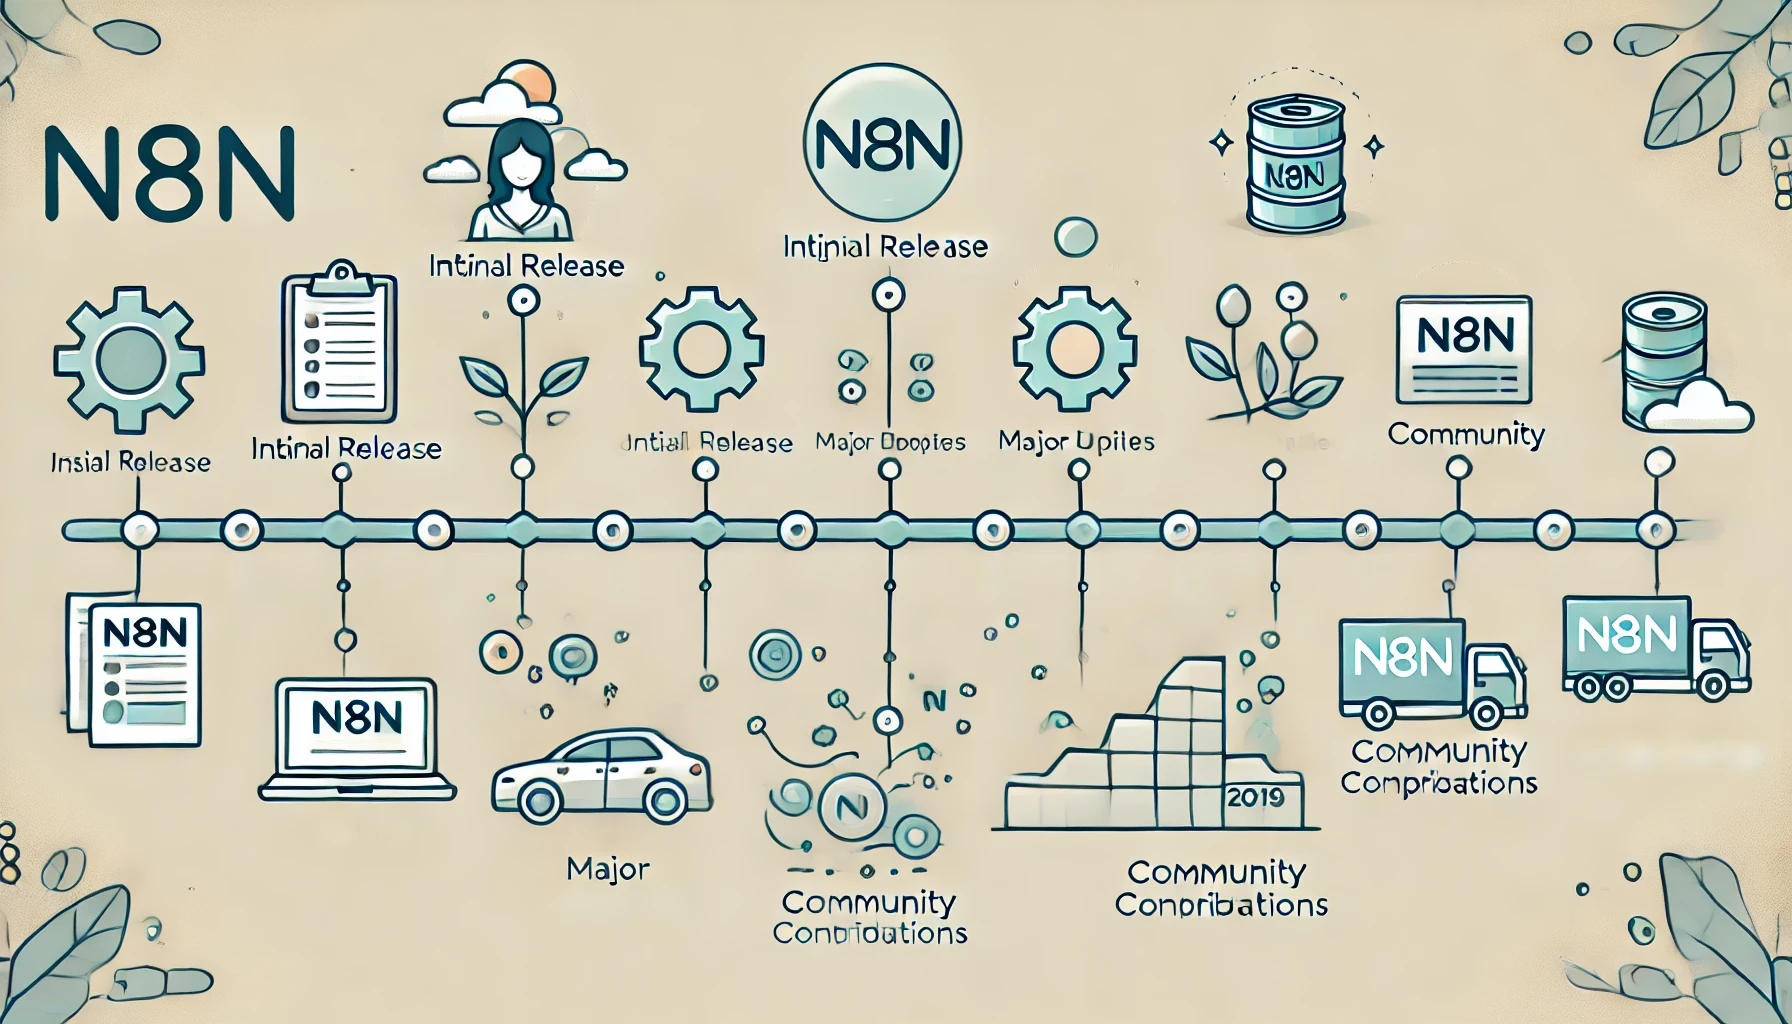
\includegraphics[width=1\linewidth]{images/history.png}
\end{figure}

\textbf{Sự khác biệt đến từ tư duy mở}

Ngay từ khi hình thành, n8n đã chọn cho mình một con đường rất riêng: mã nguồn mở, hoàn toàn có thể tự lưu trữ, và không ràng buộc người dùng vào một hệ sinh thái đóng.

Điều đó có nghĩa là gì? Có nghĩa là bạn có thể triển khai n8n trên bất kỳ máy chủ nào – từ chiếc Raspberry Pi nhỏ bé đến một hệ thống cloud khổng lồ. Bạn có thể tích hợp hơn 200 dịch vụ phổ biến, hoặc gọi bất kỳ API nào bạn muốn. Bạn có thể chỉnh sửa logic, viết JavaScript, thêm node tùy biến. Không giới hạn. Không phụ thuộc. Không đánh đổi quyền riêng tư.

$\Rightarrow$ \textit{N8N trao cho bạn chìa khóa để điều khiển luồng dữ liệu – theo cách của riêng bạn.}

Hãy nhớ lại lần cuối bạn phải thủ công sao chép dữ liệu từ Excel sang email, hay mất hàng giờ kiểm tra thông báo rải rác trên nhiều nền tảng. n8n không chỉ giúp bạn làm những việc đó - nó làm chúng nhanh hơn, thông minh hơn, và thậm chí có thể đưa ra quyết định thay bạn. Đây không chỉ là công cụ tự động hóa, mà là chìa khóa mở ra một cách làm việc mới, nơi công nghệ không thay thế con người, mà nâng tầm khả năng của chúng ta.

$\Rightarrow$ \textit{N8N không chỉ giúp bạn làm việc hiệu quả hơn. Nó thay đổi cách bạn suy nghĩ về công việc.}
        
\newpage
\section{Low-code và No-code}
Trong suốt hàng thế kỷ qua, phần mềm đã hoàn toàn thay đổi cách chúng ta làm việc và sinh hoạt. Những hệ thống đắt đỏ và cồng kềnh vốn chỉ dành cho khoa học và nghiên cứu giờ đấy đã trở nên phổ biến như xe cộ bên đường, thật chí nó còn dày đặc hơn thế. Giờ đây, chúng ta có thể làm việc với những người cách chúng ta một vòng trái đất một cách dễ dàng như việc trao đổi bài tập với lũ bạn trên đường. 

Những hệ thống này đã thay đổi xã hội hiện đại nhờ khả năng tự động hóa các nhiệm vụ phức tạp cồng kềnh và xử lý dữ liệu một cách nhất quán. Thay vì phải viết thư tay, dán tem, gửi qua bưu điện và người nhận sẽ có nó trong một vài ngày. Nhờ vào hạ tầng công nghệ hiện đại giờ đây việc gửi một bức thư chỉ diễn ra trong vòng một tích tắc.


Để xây dựng các hệ thống như vậy, trước đây bạn phải học một ngôn ngữ lập trình và thực sự làm chủ nó để viết các đoạn mã hệ thống. Việc này đòi hỏi tính kiên trì, học thuật, logic. Chúng mất quá nhiều thời gian và công sức. Một lựa chọn khác khá phổ biến hiện nay là thuê ngoài. Đơn giản nghe vẻ hợp lý nhưng bạn thử nghĩ bạn đi đâu để tìm một kĩ sư phù hợp và bạn có thực sự đủ tiền để trả cho kĩ sư đó. Để giải quyết khó khăn này các ứng dụng lowcode, nocode ra đời như một sự kiện tất yếu.

\begin{figure}[htbp]
    \centering
    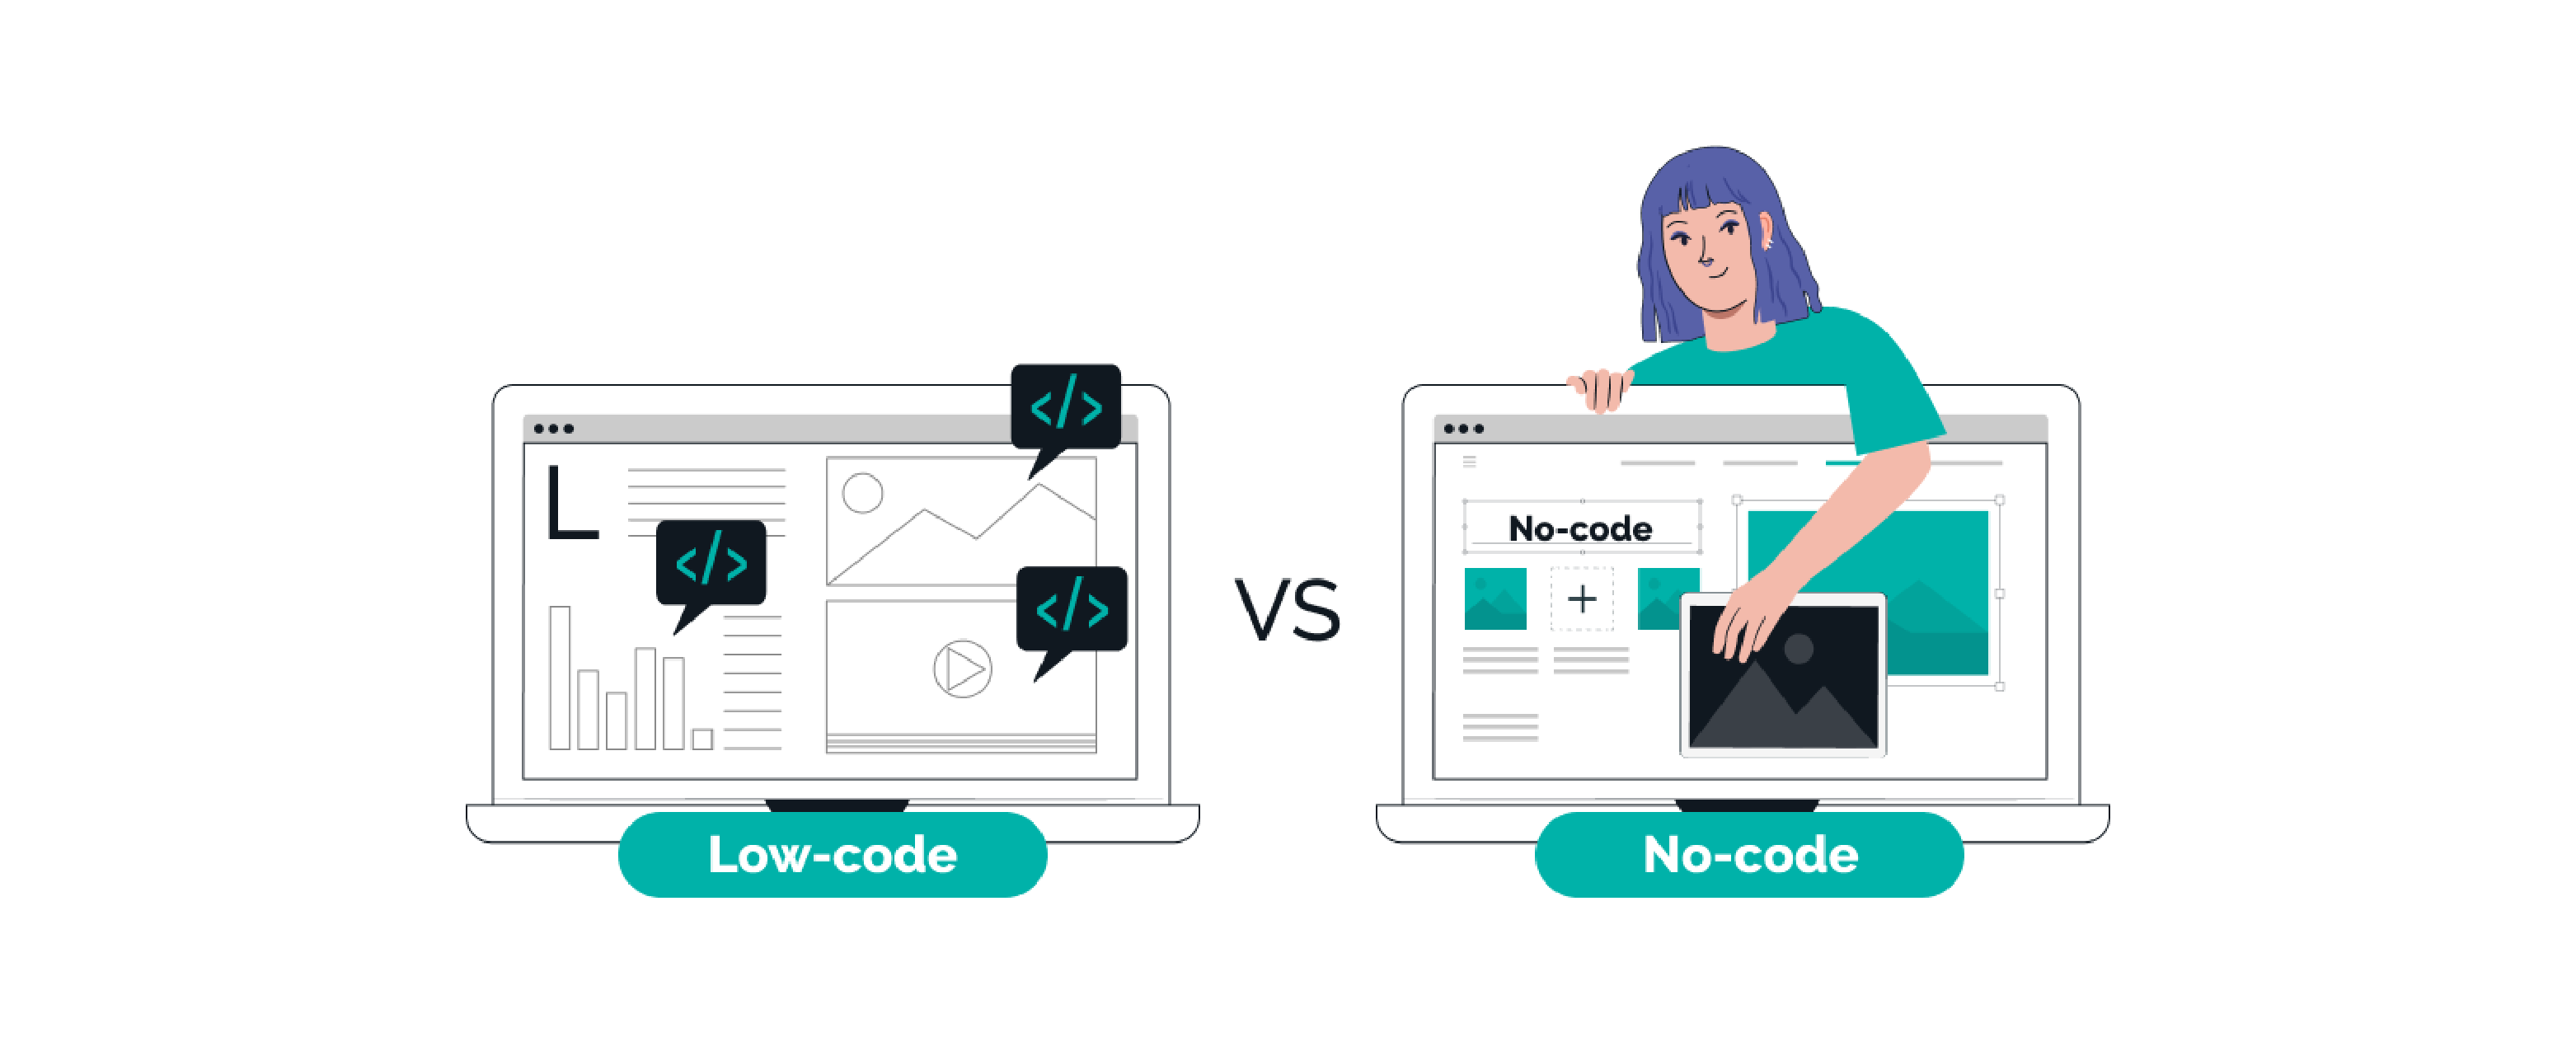
\includegraphics[width=1\linewidth]{Chap1-7/cover-Low-Code.pdf}
\end{figure}

Khi muốn tự động hóa quy trình, chúng ta sẽ nghĩ ngay đến việc dùng phần mềm. Nhưng để có phần mềm, thường phải viết code – mà code thì rắc rối, phức tạp, đòi hỏi các lập trình viên phải vắt óc suy nghĩ, gõ bàn phím đến mức "đầu bù tóc rối", thậm chí có nguy cơ hói sớm :):)

\newpage
Việc này tạo ra rào cản lớn cho tự động hóa:
\begin{itemize}
    \item Cần nhiều thời gian, công sức để học và viết code.

    \item Khi quy trình thay đổi, lại phải chỉnh sửa code, tốn kém và mất thời gian.

    \item Doanh nghiệp lớn có đội ngũ kỹ thuật thì không sao, nhưng doanh nghiệp nhỏ sẽ phải thuê ngoài, chi phí không hề nhỏ.
\end{itemize}

\textbf{Low-code vs No-code}
\begin{itemize}
    \item Low-code: Cắt giảm đáng kể lượng code. Thay vì phải viết từ A đến Z, giờ đây chỉ cần kéo thả là chính, chỉ khi cần tính năng đặc biệt mới phải viết một chút code.

    \item No-code: Hoàn toàn không cần code, chỉ kéo thả là có thể tạo ra phần mềm.
\end{itemize}

\textbf{Tranh cãi xung quanh "no code"}

Với nhiều kỹ sư kỳ cựu, các công cụ no - code từng bị xem nhẹ như một món vũ khí… thiếu sát thương – dễ dùng, nhưng không đủ lực để giải quyết bài toán phức tạp. Sử dụng no - code đôi khi bị ngầm hiểu là dấu hiệu của một kỹ sư "non tay". Chẳng hạn, các công cụ ETL dạng kéo-thả như Talend – một nhóm yêu thích vì dễ dùng, nhóm khác lại chê vì khó mở rộng và thiếu linh hoạt trong xử lý hàng loạt.

Quan điểm này từng có lý, nhất là khi no-code còn sơ khai. Nhưng vài năm trở lại đây, ranh giới giữa no-code và code đã mờ dần. Khi các nền tảng no-code ngày càng mạnh mẽ và linh hoạt hơn, giá trị thực tế mà chúng mang lại cho doanh nghiệp không thể xem thường. Không còn là giải pháp "tạm bợ", no - code đang dần trở thành lựa chọn chiến lược.


\textbf{N8N: Vừa Low-code vừa No-code}

N8N là ví dụ điển hình cho làn sóng mới này. Nó không thuần no-code, cũng không ép người dùng phải code như một lập trình viên chuyên nghiệp. Với các workflow đơn giản, bạn có thể kéo – thả mà không cần viết dòng nào. Nhưng khi cần tự do hơn, bạn hoàn toàn có thể nhúng vài đoạn mã nhỏ – dễ hiểu, dễ sửa, và không hề phức tạp như xây một hệ thống từ con số 0.

$\Rightarrow$ \textit{Nói cách khác, N8N giúp bạn tự động hóa nhanh chóng mà không cần là dân lập trình chuyên nghiệp.}




\newpage
\section{Tại sao nên học n8n?}

% Từ thời chinh chiến nơi giảng đường đại học, hằng ngày lòa mắt với từng con số phép tính vi phân, tích chập. Học mãi chẳng vào vì chúng quá là phức tạp. Tư duy mãi cũng ko biết làm, thi mãi điểm cũng chả cao, rồi chán rồi nản. Ở đây n8n không thế, nó cực kỳ easy cho người mới bắt đầu ko nhất thiết phải có tí tech tủng trong người mà vẫn tung hoành thiên hạ được. 
Hồi còn “chinh chiến” nơi giảng đường, ngày ngày vật lộn với vi phân, tích chập, những con số như nhảy múa trước mắt. Học mãi không vào, làm mãi chẳng ra, thi xong nhìn điểm mà muốn xỉu. Tưởng chừng như công nghệ hay tự động hóa là thứ gì đó xa vời, chỉ dành cho những người giỏi kỹ thuật.

\begin{figure}[htbp]
    \centering
    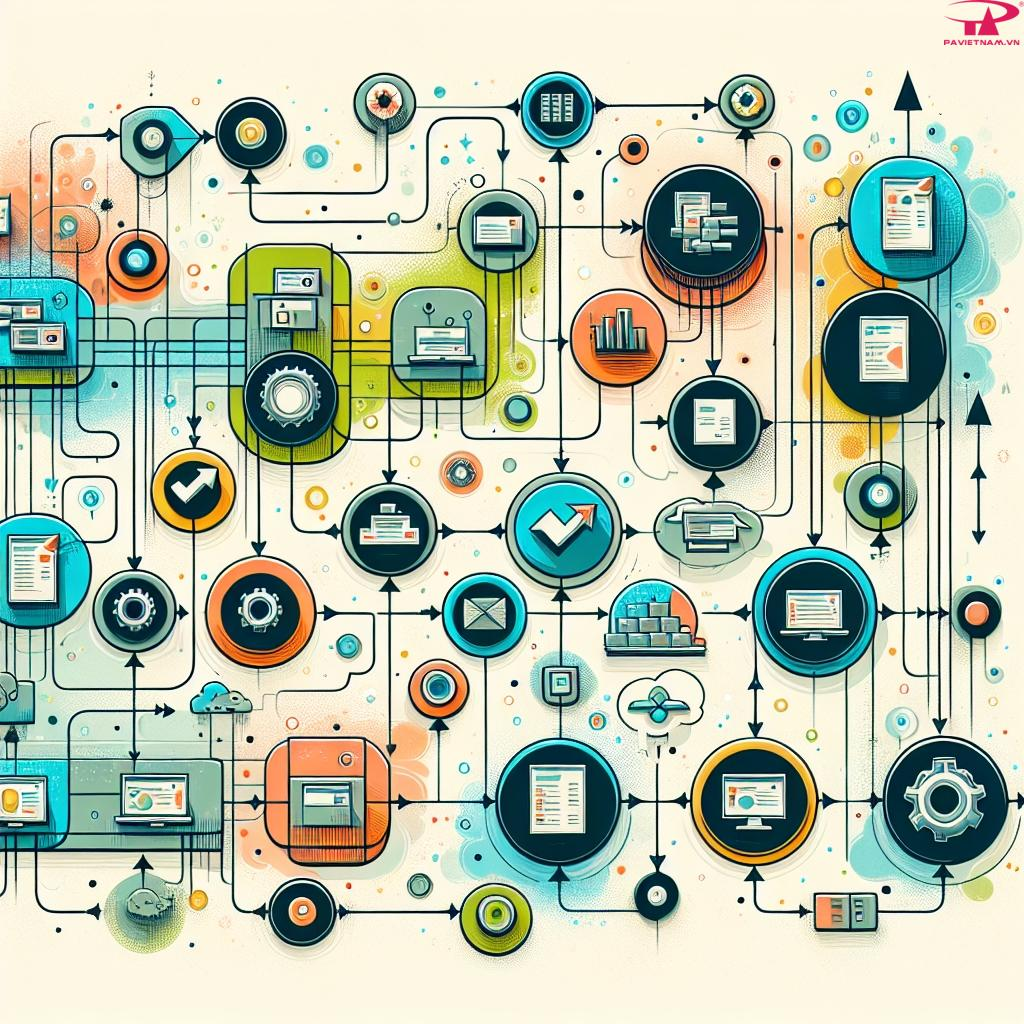
\includegraphics[width=1\linewidth]{images/wf.jpg}
    \caption{Minh họa các node}
\end{figure}

Nhưng rồi mình gặp n8n.

Một nền tảng tự động hóa thân thiện đến không ngờ. Không cần giỏi lập trình, không cần "máu tech", chỉ cần một chút tò mò và sự kiên nhẫn là đã có thể bắt đầu tạo ra những quy trình tự động giúp cuộc sống và công việc nhẹ nhàng hơn hẳn. Với n8n, bạn có thể "làm điều lớn" mà không cần "kiến thức lớn".

Học n8n không giống như học code kiểu truyền thống — nó gần giống như chơi lego, ráp từng mảnh nhỏ thành một hệ thống tự động hóa hoàn chỉnh. Và chính cảm giác "tự tay làm được" ấy mới khiến mình mê mẩn n8n đến vậy.

Như tôi nói ở trên ấy, n8n chỉ việc set up rồi chỉ việc tư duy để kéo thả qua các node (node là gì nói sau). Không phải cầu kỳ như dân dev 

Tự động hóa - Chìa khóa để trở thành doanh nghiệp dựa trên dữ liệu. Quan sát thử bảng sau:

\begin{table}[h]
    \centering
    \renewcommand{\arraystretch}{1.5}
    \begin{tabular}{| m{6cm} | m{6cm} |}
        \hline
        \textbf{Công việc thủ công} & \textbf{Tự động hóa} \\
        \hline
        Lãng phí thời gian & Tính dự đoán cao \\
        \hline
        Lỗi do con người (các nhiệm vụ lặp đi lặp lại có giá trị thấp) & Cải thiện khả năng truy cập dữ liệu - Tăng ROI lên nhiều\\
        \hline
        Yêu cầu nhiều nhân lực & Tăng hiệu suất làm việc của nhân viên \\
        \hline
        Nhân viên ít hạnh phúc và khó giữ chân & Tập trung vào các nhiệm vụ có giá trị cao hơn \\
        \hline
    \end{tabular}
    \caption{So sánh giữa Công việc thủ công và Tự động hóa}
\end{table}

\textbf{Tôi tóm gọn trong 5 lý do sau này:}

\begin{itemize}
    \item Giá rẻ và mã nguồn mở - không tốn phí subscription như Zapier hay Make, phù hợp để học và thử nghiệm
    \item Dễ học với giao diện trực quan - kéo thả node để tạo workflow, không cần code nhiều
    \item Tự do kiểm soát, riêng tư - có thể tự host, quản lý dữ liệu và customize theo ý muốn
    \item Đa năng và mạnh mẽ - tích hợp được nhiều service, chạy được code JavaScript/Python, xây dựng được các workflow phức tạp
    \item Kỹ năng hot - automation đang nổi lên như một xu hướng, biết n8n sẽ tăng giá trị CV và cơ hội nghề nghiệp của bản thân
    \item Hỗ trợ hơn 200 tích hợp sẵn: Kết nối với các dịch vụ phổ biến như Google, Slack, Twitter, v.v.
\end{itemize}

\section{n8n ở đâu trước cơn hót trend Automation}

% Các đối thủ như Zapier, Make là các giải pháp độc quyền, hosting tập trung và tính phí theo subscription

% \begin{itemize}
%     \item Zapier: Hạn chế về tính linh hoạt, chỉ hỗ trợ một số tính năng nhất định, chủ yếu dựa trên các workflows đơn giản.
%     \item n8n: Linh hoạt hơn rất nhiều, hỗ trợ custom code, dễ dàng kết nối API và xử lý các workflows phức tạp.
%     \item Integromat (Make): Tương tự như n8n, nhưng n8n miễn phí mã nguồn mở và có tính năng tùy chỉnh sâu hơn.
% \end{itemize}

Trên thị trường nền tảng tự động hóa, những cái tên như Zapier hay Make từ lâu đã trở thành lựa chọn quen thuộc với người dùng nhờ giao diện thân thiện và khả năng triển khai nhanh. Tuy nhiên, cả hai đều là các nền tảng độc quyền, lưu trữ tập trung trên cloud, và tính phí theo mô hình subscription – điều này có thể khiến doanh nghiệp phải phụ thuộc vào hạ tầng và định giá của bên thứ ba trong suốt quá trình sử dụng.

\begin{itemize}
    \item Zapier – tuy nổi tiếng vì dễ dùng, nhưng lại khá hạn chế về tính linh hoạt. Hầu hết người dùng chỉ có thể sử dụng các bước workflow đơn giản với tập hợp chức năng giới hạn. Zapier không cho phép can thiệp sâu bằng code, khiến việc xử lý các tác vụ phức tạp trở nên khó khăn hoặc không khả thi.

    \item Make – được đánh giá cao hơn Zapier về mức độ tùy chỉnh và khả năng xử lý các quy trình tự động hóa phức tạp. Tuy nhiên, Make vẫn là một nền tảng độc quyền với chi phí sử dụng có thể tăng nhanh khi mở rộng quy mô. Việc triển khai hoàn toàn phụ thuộc vào hệ thống cloud của họ, khiến người dùng không thể kiểm soát hoặc host cục bộ nếu cần.
    \item Khác biệt với hai đối thủ trên, n8n chọn một hướng đi táo bạo: mã nguồn mở, có thể host tại chỗ, miễn phí và cực kỳ linh hoạt. Người dùng không chỉ có thể kéo – thả để xây workflow đơn giản, mà còn dễ dàng nhúng custom code, gọi REST API, xử lý dữ liệu nâng cao và tích hợp với các hệ thống phức tạp. Với n8n, việc mở rộng quy trình hay kiểm soát luồng dữ liệu không còn là điều “bất khả thi” như ở các nền tảng đóng.

\end{itemize}
Thêm vào đó, vì là mã nguồn mở, n8n cho phép người dùng can thiệp vào logic hệ thống, tùy chỉnh sâu theo nhu cầu nội bộ mà không bị ràng buộc bởi giới hạn của nhà cung cấp. Đây là một lợi thế chiến lược với các đội ngũ kỹ thuật muốn tiết kiệm chi phí dài hạn, đồng thời đảm bảo quyền kiểm soát tuyệt đối với hệ thống của mình.




\section{n8n có thể làm được gì?}

n8n là một công cụ hoạt động trên nền tảng web, có thể chạy trên các thiết bị nhỏ gọn và giá rẻ như Raspberry Pi. Nó có thể kết nối với hàng trăm hệ thống khác nhau thông qua các node được thiết kế riêng, cũng như hàng nghìn hệ thống khác thông qua REST API tiêu chuẩn.

n8n không chỉ có khả năng chuyển đổi và xử lý dữ liệu, mà còn có thể thực hiện phân tích dữ liệu để cung cấp những thông tin hữu ích. Vì có thể tích hợp với hầu hết các hệ thống có API, nên khả năng của n8n chỉ bị giới hạn bởi những hệ thống mà nó kết nối.

Ví dụ:
\begin{itemize}
    \item Bạn muốn tạo hình ảnh 3D tự động? Có một API cho việc đó.

    \item Bạn muốn remix nhạc theo màu sắc mà webcam thu thập? Bạn có thể tạo một workflow để làm điều này.
    
    \item Bạn muốn n8n tự động cân đối sổ sách và hiển thị tình hình tài chính theo thời gian thực? Điều đó hoàn toàn có thể.

    \item Nếu có cách để kết nối n8n với một hệ thống, thì n8n có thể kế thừa sức mạnh của hệ thống đó.
\end{itemize}
